%\documentclass[a4paper,10pt]{report}
\documentclass{report}
\usepackage[utf8x]{inputenc}    
\usepackage[T1]{fontenc}
\usepackage[francais]{babel}     
\usepackage{verbatim}
\usepackage{graphicx}
\usepackage{float}
\usepackage{makeidx}
\usepackage{moreverb}
\usepackage{listings}
\usepackage{color}
\usepackage{xcolor}
\usepackage{hyperref}
\usepackage[top=2.5cm,bottom=2.5cm,right=2.5cm,left=2.5cm]{geometry}
\usepackage{here}

\definecolor{mygreen}{rgb}{0,0.6,0}
\definecolor{mygray}{rgb}{0.5,0.5,0.5}
\definecolor{mymauve}{rgb}{0.58,0,0.82}

\lstset{ %
   backgroundcolor=\color{white},   % choose the background color; you must add \usepackage{color} or \usepackage{xcolor}
   basicstyle=\footnotesize,        % the size of the fonts that are used for the code
   breakatwhitespace=false,         % sets if automatic breaks should only happen at whitespace
   breaklines=true,                 % sets automatic line breaking
   captionpos=b,                    % sets the caption-position to bottom
   commentstyle=\color{mygreen},    % comment style
   deletekeywords={...},            % if you want to delete keywords from the given language
   escapeinside={\%*}{*//)},          % if you want to add LaTeX within your code
   extendedchars=true,              % lets you use non-ASCII characters; for 8-bits encodings only, does not work with UTF-8
   frame=single,                    % adds a frame around the code
   keepspaces=true,                 % keeps spaces in text, useful for keeping indentation of code (possibly needs columns=flexible)
   keywordstyle=\color{blue},       % keyword style
   language=Octave,                 % the language of the code
   morekeywords={*,...},            % if you want to add more keywords to the set
   numbers=left,                    % where to put the line-numbers; possible values are (none, left, right)
   numbersep=5pt,                   % how far the line-numbers are from the code
   numberstyle=\tiny\color{mygray}, % the style that is used for the line-numbers
   rulecolor=\color{black},         % if not set, the frame-color may be changed on line-breaks within not-black text (e.g. comments (green here))
   showspaces=false,                % show spaces everywhere adding particular underscores; it overrides 'showstringspaces'
   showstringspaces=false,          % underline spaces within strings only
   showtabs=false,                  % show tabs within strings adding particular underscores
   stepnumber=2,                    % the step between two line-numbers. If it's 1, each line will be numbered
   stringstyle=\color{mymauve},     % string literal style
   tabsize=2,                       % sets default tabsize to 2 spaces
   title=\lstname                   % show the filename of files included with \lstinputlisting; also try caption instead of title
}
\lstset{language=C,caption={Projet A13 LO41}}%,label=DescriptiveLabel}

\hypersetup{
     bookmarks=true,         % show bookmarks bar?
     unicode=true,          % non-Latin characters in Acrobat’s bookmarks
     pdftoolbar=true,        % show Acrobat’s toolbar?
     pdfmenubar=true,        % show Acrobat’s menu?
     pdffitwindow=false,     % window fit to page when opened
     pdfstartview={FitH},    % fits the width of the page to the window
     pdftitle={Projet LO41},    % title
     pdfauthor={Yoann CAPLAIN},     % author
     pdfsubject={Une chaîne de montage},   % subject of the document
     pdfcreator={Yoann CAPLAIN},   % creator of the document
     pdfproducer={Producer}, % producer of the document
     pdfkeywords={LO41} {CAPLAIN} {A13}, % list of keywords
     pdfnewwindow=true,      % links in new window
     colorlinks=true,       % false: boxed links; true: colored links
     linkcolor=black,          % color of internal links (change box color with linkbordercolor)
     citecolor=green,        % color of links to bibliography
     filecolor=magenta,      % color of file links
     urlcolor=cyan           % color of external links
}

\begin{document}
\begin{figure}[!p!t]

\includegraphics[height=60pt]{utbm.png}
\end{figure}

\title{Projet LO41\\ \huge{\textbf{Une chaîne de montage en anneau}}}
\author{Yoann \bsc{Caplain}}
\date{\today \\Semestre A2013}


\maketitle \clearpage 
\tableofcontents %\clearpage

%\part{Partie}
\chapter{Introduction}
Dans le cadre de l’unité de valeur “LO41 : Système d'exploitation : Principes et Communication”, il nous est demandé de réaliser un projet permettant d’appliquer les différents concepts étudiés tout au long des cours, travaux pratiques et travaux dirigés. Le projet “Chaîne de montage en anneau” qui nous a été soumis permet de mettre en oeuvre ces concepts.
\section{Rappel du sujet : La chaîne de montage en anneau}
Le but du projet est de réaliser un approvisionnement de composants matériels et la gestion du processus de fabrication d'une gamme de produits.\\
On doit mettre en oeuvre une chaîne de montage "en anneau" pilotée par des robots, sa particularité est que la chaîne a 16 sections pouvant contenir soit des composants servant à la fabrication de produit, des produits en cours de fabrication ou des produits finaux.\\
Ces robots sont au nombre de 6 et ont deux modes différents (mode normal et dégradé), ils ont chacun leurs caractéristiques propres (opération normal et opérations en mode dégradé).\\
Les composants servent à créer le produit (1ère opération du produit).\\\\
Le projet doit être codé en C et utilisé l'une (ou plusieurs) des méthodes de synchronisation vu en cours:
\begin{itemize}
\item Mutex
\item Mémoire partagée
\item Flux (tubes)
\item Sémaphore
\item etc
\end{itemize}
\section{Analyse du sujet}
\subsection{Les composants}
Un composant sert juste à créer un produit et ils sont utilisés lors de la 1ère opération, ils sont donc liés aux opérations et un seul type de composant est nécessaire pour créer un produit.\\
On a 4 composants différents:
\begin{itemize}
\item C1
\item C2
\item C3
\item C4
\end{itemize}
\subsection{Les opérations}
Les opérations sont des actions réalisées par les robots.\\
En mode normal une opération n'est faite que par un seul robot contrairement au mode dégradé où une opération peut être liée à plusieurs robots.\\
On a 6 opérations différentes:
\begin{itemize}
\item Op1
\item Op2
\item Op3
\item Op4
\item Op5
\item Op6
\end{itemize}
\subsection{Les produits}
Pour créer un produit il faut les composants nécessaires pour la 1ère opération du produit, les opérations suivantes n'ont pas besoin d'utiliser de composants.\\
On a 4 produits différents (et leur séquence):
\begin{itemize}
\item Prod1 (Op1, Op2, Op3, Op5)
\item Prod2 (Op2, Op4, Op1, Op6)
\item Prod3 (Op3, Op1, Op5, Op1, Op3)
\item Prod4 (Op4, Op6, Op1)
\end{itemize}
\subsection{L'anneau}
L'anneau est circulaire et possède 16 sections qui peuvent stocker des composants et des produits.\\
L'anneau est accédé par les robots (6 robots), la chaîne d'approvisionnement des composants et la chaîne de sortie des produits finis.
\subsubsection{Algorithme de l'anneau}
L'algorithme décrit ci-dessous montre principalement comment ça se passe pour le code, il y a certaines parties du code omis volontairement ici.
\begin{lstlisting}[caption=Algorithme de l'anneau simplifié]
Tant que continuer
	Lock mutex anneau
	Tant que qqChoseAccedeAnneau > 0
		Attendre sur condition 'Acces a anneau'
	Fin Tant que
	Tourner l''anneau
	Signaler tous ceux qui attendent sur la condition que 'Anneau a tourne'
	Unlock mutex anneau
Fin Tant que
\end{lstlisting}

\subsection{Les robots}
Les robots accèdent à l'anneau pour récupérer des composants ou des produits non finis, ils y déposent seulement des produits.\\
Ils créent des produits à partir des composants stockés.
\subsubsection{Les modes des robots}
Les robots ont deux modes qui sont Normal et Dégradé.\\
En mode normal les robots n'ont qu'une seule opération disponible, en mode dégradé ils ont la possibilités de réaliser plusieurs opérations.
\subsubsection{Algorithme des robots}
L'algorithme décrit ci-dessous montre principalement comment ça se passe pour le code, il y a certaines parties du code omis volontairement ici.\\
Dans cet algorithme les mutex ne seront pas décrit.
\begin{lstlisting}[caption=Algorithme des robots simplifié]
Tant que continuer
	Attendre sur condition que 'Anneau a tourne'
	Si le robot peut creer le produit Alors
		Creer le produit
	Sinon
		Si l''emplacement de l''anneau pour le robot est un composant Alors
			Si le composant est utile pour le robot Alors
				Prendre le composant
			Fin si
		Sinon si l''emplacement de l''anneau pour le robot est un produit Et que le robot ne possede pas deja un produit Alors
			Si l''operation suivante peut etre faite Alors
				On prend le produit et on fait l''operation
			Fin si
		Fin si

		Si l''emplacement de l''anneau pour le robot est vide
			Si le robot a besoin de poser un produit
				Poser le produit sur l''anneau
			Fin si
		Fin si
	Fin si
	Signaler Anneau sur condition 'Acces a anneau'
Fin Tant que
\end{lstlisting}

\chapter{Analyse et conception}
\section{UML : Langage de modélisation}
L'analyse d'un projet est primordiale, ça permet de clarifier les aspects techniques et ce que l'on veut faire sur notre projet. C'est pourquoi cette analyse est très importante et qu'il faut qu'elle soit correct avant le début de la conception du projet car selon l'erreur d'analyse celle-ci peut soit être résolu avec quelques modifications ou nécessite de recommencer la conception du projet.\\


L'analyse qui a été faite sur le projet Chaîne de montage en anneau a permis de mettre en place une struture du programme futur.\\
En sachant que l'UML est orientée objet il a été utilisé que pour clarifier le projet et voir quels vont être les fichiers sources du programme.\\
De plus cette analyse a été faite de façons à avoir un code modulable grâce aux factory et une abstraction de la représentation des produits, des composants et des opérations.
\newpage
\subsection{Le diagramme de classe}
Le diagramme de classe a été la base du projet, certaines classes vu ci-dessous ne sont pas dans le projet étant donné que c'était une 1ère approche du projet et qu'une adaptation en C (non orientée objet) était nécessaire, aussi les "factory" ne sont pas représentées.
\begin{figure}[H]
\center
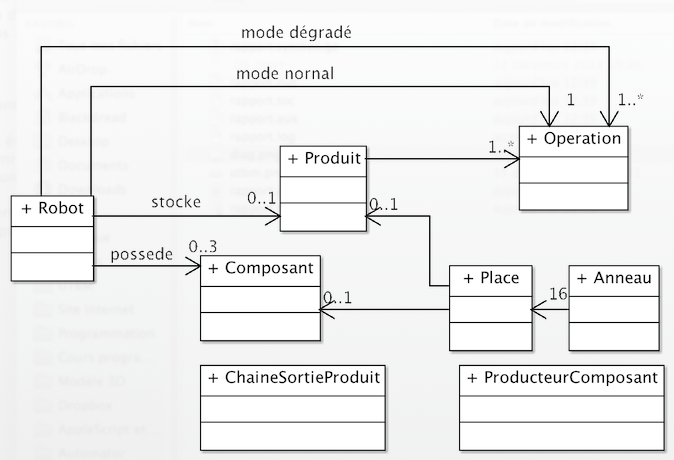
\includegraphics[width=400pt]{diag.png}
\caption{Diagramme de classe}
\label{Diagramme de classe}
\end{figure}

\chapter{Réalisation du projet}
\section{Structure générale}
Le programme est réalisé en C et la synchronisation est faite avec des mutex sur les thread.
\section{Description des fichiers sources}
La plupart des fichiers sources sont commentés donc nous ne ferons pas forcément de descriptions complètes pour certaines de ces sources.\\
De plus les fichiers .c ne seront pas dans le rapport étant donné le volume de ligne que cela représente, voir le code source donné à part du rapport (ou cf \ref{realisation} page \pageref{realisation}).
\subsection{Anneau}
Il y a un mutex (mutex\_anneau) et deux conditions (cond\_anneauATourner, cond\_anneauAttenteAcces).
Le mutex permet la synchronisation sur l'anneau pour tout les éléments qui veulent y accèder.
La 1ère condition permet de notifier ceux qui attendent que l'anneau est tourné. La 2ème condition permet de réveiller l'anneau dès qu'un élément à fini d'accèder à l'anneau, celui-ci est réveillé et vérifie s'il y a encore des éléments qui accède à l'anneau si oui il se rendort sinon il tourne.

La définition des emplacements des robots, chaîne entrée et chaîne sortie se trouvent ici. L'initiation de l'anneau se fait avec la fonction "initAnneau".
\begin{lstlisting}[caption=Représentation de l'anneau]
#ifndef LO41__anneauCircu
#define LO41__anneauCircu

#include <stdio.h>
#include <stdlib.h>
#include <pthread.h>
#include "Robots.h"
#include "Produit.h"
#include "ProducteurComposant.h"

#define TAILLE_ANNEAU_MAX 16

#define POS_C_ENTREE 1
#define POS_C_P_SORTIE 3
#define POS_ROBOT_1 5
#define POS_ROBOT_2 7
#define POS_ROBOT_3 9
#define POS_ROBOT_4 11
#define POS_ROBOT_5 12
#define POS_ROBOT_6 14

#define TYPE_PROD 50
#define TYPE_COMP 51
#define TYPE_RIEN 0

pthread_mutex_t mutex_anneau;
// Permet de reveiller robots et autres en attente
pthread_cond_t cond_anneauATourner;

// l'anneau attend tant que les elements continue d'acceder a l'anneau
pthread_cond_t cond_anneauAttenteAcces;

void initAnneau();

int bufComposantOuProduit[TAILLE_ANNEAU_MAX]; // 51 c et 50 Prod <= ce n'est pas forcement utile car on peut supposer que tout les pointeur de type produit auront une valeur superieur a 1000 donc on pourrait juste tester la valeur du pointeur, mais qui a faire bien je mets ce 2eme tableau
void *bufferAnneau[TAILLE_ANNEAU_MAX];

void* prendreElement(int positionBuffer);
void ajouterElement(void *elem,int positionBuffer,int type);
int isPostionBufLibre(int pos);
int getPositionType(int pos);

// renvoie la position du robot sur le buffer
int getPositionDuRobot(int numRobot);

// Ne pas trop utiliser cette fonction
void* getPointeur(int pos);

int continuerAnneau;

int nbElementDansBuffer;

int nbElementQuiAccedeAnneau;
//int nbElementQuiVeulentAccedeAnneau;

void printAnneau();

void th_tournerAnneau();

#endif
\end{lstlisting}
\begin{figure}[H]
\center
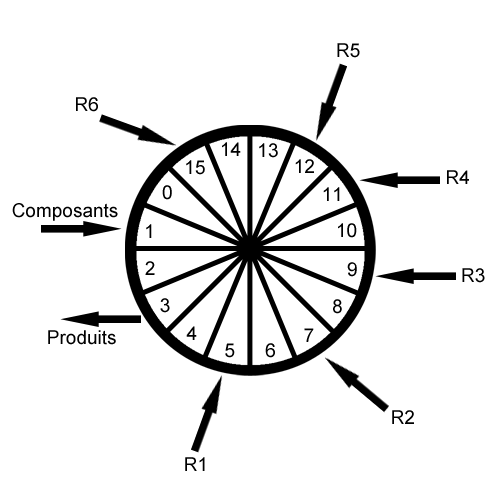
\includegraphics[width=200pt]{chaineMontage.png}
\caption{Aperçu de l'anneau}
\label{diagSeq}
\end{figure}
L'anneau est l'élément critique du projet:
\begin{itemize}
\item Attendre qu'aucun élément accède l'anneau
\item Tourner (déplacer les éléments d'un cran)
\item Notifier ceux qui attendent que l'anneau est tourné
\item Recommencer
\end{itemize}
\begin{lstlisting}[caption=Fonction du thread de l'anneau]
void th_tournerAnneau(){
    while(continuerAnneau == 1){

        pthread_mutex_lock(&mutex_anneau);
        while(nbElementQuiAccedeAnneau != 0){
            printf("Anneau mis en attente\n");
            pthread_cond_wait(&cond_anneauAttenteAcces, &mutex_anneau);
        }
        
        // tourne les elements
        int i;
        int tmp = bufComposantOuProduit[TAILLE_ANNEAU_MAX-1];
        void* tmp2 = bufferAnneau[TAILLE_ANNEAU_MAX-1];
        
        for(i=TAILLE_ANNEAU_MAX-1;i>0;i--){
            bufComposantOuProduit[i] = bufComposantOuProduit[i-1];
            bufferAnneau[i] = bufferAnneau[i-1];
        }
        bufComposantOuProduit[0] = tmp;
        bufferAnneau[0] = tmp2;
        //printf("Anneau a tourner\n");
        
        pthread_cond_broadcast(&cond_anneauATourner);
        pthread_mutex_unlock(&mutex_anneau);
    }
    printf("Thread Anneau terminer\n");
}
\end{lstlisting}

\subsection{Robot}
La définition du robot est une structure, on peut ainsi créer plusieurs robots à partir de cette structure. De plus la création est simplifiée et centralisée avec FactoryRobot.
\begin{lstlisting}[caption=Représentation des robots]
#ifndef LO41_Robots_h
#define LO41_Robots_h

//* ca se trouve ici car sinon dans FactoryRobot j'avais une inclusion circulaire, a corriger
#define R1 1
#define R2 2
#define R3 3
#define R4 4
#define R5 5
#define R6 6
//*/
#define TAILLE_MAX_NB_OP_DEGRADE 4
#define TAILLE_MAX_NB_COMP_GARDE 3

#define MODE_NORMAL 1
#define MODE_DEGRADE 2

#include <stdio.h>
#include <stdlib.h>
#include "Produit.h"
#include "Operation.h"
#include "Composant.h"
#include "anneauCircu.h"
#include "FactoryProduit.h"


typedef struct _robot{
    int continuer; // ajouter a la fin, c'est juste pour arreter le thread a partir du main
    int mode;
    
    int opNormal;
    
    // Nb d'element => Ou remplacer par un pointeur et garder le nb d'element de ce tableau
    int nbOpDegrade;
    int opDegrade[TAILLE_MAX_NB_OP_DEGRADE]; // taille statique ou pointeur
    
    // peut posseder un produit
    produit* produit;
    // peut posseder des composants => supposer identique car dans le sujet les produits commencent avec un seul type de composant
    int composant[TAILLE_MAX_NB_COMP_GARDE];
    
}robot;

void changerModeRobot(int mode, robot *robot);

// Regarde si le produit passer en parametre peut etre utiliser par le robot (si le robot peut faire l'operation)
int isProduitNextOpCanBeDone(produit *prod, robot *robot);

// renvoie 1 si oui. Regarde si ce composant est utile au robot ce qui signifie si ce robot peut creer un produit a partir de ce composant, ne prends que les composants d'un meme type si 1 type a deja etait pris.
int isComposantUsefulToBeTaken(int composant, robot *robot);

// renvoie 1 si le robot a deja des composants de stocke
int isRobotAlreadyHaveComposant(robot *robot);

// renvoie le nb de composant
int countNbComposant(robot *robot);

// renvoie 1 si le robot possede un produit a remettre sur l'anneau
int isRobotNeedToGiveProduit(robot *robot);

// renvoie 1 si le robot est plein de composants
int isRobotFullOfComposant(robot *robot);

// ajoute le composant -> attention a la limite en taille -> si ca depasse le composant est perdu
void ajouterComposant(int composant, robot *robot);

// supprime les composants
void enleverLesComposants(robot *robot);

// supprime un composant de type donne (part de la fin a 0)
void enleverLeComposant(int composant, robot *robot);


// Num robot et arg[1] un pointeur sur un robot
void th_robot(void* arg[]);
//void th_robot(void *numRob, robot *robot);

// la fonction qui enleve les composants, creer le produit puis...
void procederALaCreationDuProduit(int numProd, robot *robot);

// fonction qui fais les operations sur le produit (faire l'op suivante de la suivante si le robot peut le faire ? (robot en mode degrade donc))
void procederOpSuivanteDuProduit(robot *robot);

// On remet sur l'anneau le produit (toute verification faite cette fonction
void procederRemiseDuProduitSurAnneau(int positionSurAnneau, robot *robot);

#endif
\end{lstlisting}


On a une seule fonction qui permet de gérer n'importe quel robot, c'est donc modulable et le changement ne se fait que dans cette fonction, on n'a pas de code copier.\\
Et la création des différents robots se fait grâce au FactoryRobot.


Les robots vont prendre possesion du mutex, puis attendre que l'anneau est tourné, une fois qu'ils ont repris possession du mutex ils incrémentent un int pour notifier l'anneau qu'il y a des éléments qui y accède.\\
Ce que qu'ils font ensuite est la création d'un produit en vérifiant auparavant que c'est possible sinon ils regardent s'il y a quelque chose à prendre sur l'anneau (à l'emplacement qu'il leur a été assigné) soit c'est vide soit c'est un composant soit c'est un produit.\\
Suivant ce que c'est, pour le cas où c'est un composant, ils le prendront et s'ils ont un produit à déposer aussi ils vont le déposer tout en prenant l'élément sur l'anneau, ainsi on ne perd pas de temps.


L'algorithme permet aussi à un robot de faire plusieurs opérations sur un produit sans le remettre sur l'anneau si les opérations suivantes sont faisables par le robot.
\begin{lstlisting}[caption=Fonction thread des robots]
void th_robot(void* arg[]){
//void th_robot(void *numRob, robot *robot){
    robot *robot = arg[1];
    int numRobot = (int)arg[0];
    
    while(robot->continuer == 1){
        pthread_mutex_lock(&mutex_anneau);
        // On attend tjr que l'anneau est tournee
        pthread_cond_wait(&cond_anneauATourner, &mutex_anneau);
        nbElementQuiAccedeAnneau++;
        
        // ******************* ALGO *******************
        // regarder si on veut prendre des composants
        // regarder le composant -> on le prends ?
        // on prend le composants si on a en a besoin pour creer un produit (produit qui a besoin de plusieurs compo)
        // Besoin que de 1 composant -> ce composant nous est presente => on le prends et on creer le produit
        
        // regarder le produit -> possible de faire l'action ?
        // possible mais pas les composants, on atttends les prochains composants
        // possible et ce n'est pas la 1ere op donc on fait l'op
        // ******************* ALGO *******************
        
        
        int nbCompo = countNbComposant(robot);
        int numProdACreer = 0;
        //if(nbCompo > 0)
            numProdACreer = hasEnoughComposantToDoProd(nbCompo, robot->composant[0]);
        if(nbCompo > 0 && numProdACreer > 0 && isRobotNeedToGiveProduit(robot) == 0){
            // supposition -> un seul type de composant
            nbElementQuiAccedeAnneau--;
            pthread_cond_signal(&cond_anneauAttenteAcces);
            pthread_mutex_unlock(&mutex_anneau);
            
            printf("Robot%d procede creation produit\n", numRobot);
            procederALaCreationDuProduit(numProdACreer, robot);
            
            continue;
        }else{
        
            pthread_mutex_unlock(&mutex_anneau);
            int typePos = getPositionType(getPositionDuRobot(numRobot));
            
            if(typePos == TYPE_COMP){
                int composantSurAnneau = (int)getPointeur(getPositionDuRobot(numRobot));
                
                // On ne peut pas encore creer de produit => on cherche a avoir les composants necessaires
                if(isRobotAlreadyHaveComposant(robot) == 1){
                    // Un produit n'a besoin que d'1 type de composant donc on ne va pas chercher a stocker differents composant
                    if(composantSurAnneau == robot->composant[0] && isRobotFullOfComposant(robot) == 0){
                        // on prend le composant
                        ajouterComposant((int)prendreElement(getPositionDuRobot(numRobot)), robot);
                        typePos = TYPE_RIEN;
                        printf("Robot%d pris composant %d 1er nb=%d\n", numRobot,composantSurAnneau,countNbComposant(robot));
                    }
                }else{
                    // on prend le composant seulement si utile pour ce robot
                    if(isRobotFullOfComposant(robot) == 0 && isComposantUsefulToBeTaken(composantSurAnneau,robot) == 1){
                        ajouterComposant((int)prendreElement(getPositionDuRobot(numRobot)), robot);
                        typePos = TYPE_RIEN;
                        printf("Robot%d pris composant %d 2eme nb=%d\n", numRobot,composantSurAnneau,countNbComposant(robot));
                    }
                }
            }else if(typePos == TYPE_PROD && isRobotNeedToGiveProduit(robot) == 0){
                produit* produitSurAnneau = (produit*)getPointeur(getPositionDuRobot(numRobot));
                if(isProduitNextOpCanBeDone(produitSurAnneau, robot) == 1){
                    // on peut faire l'operation
                    // regarder si on peut faire plusieurs op si on est en mode degrade, c bete de remettre le produit si on peut faire les 2 operations qui suivent
                    robot->produit = prendreElement(getPositionDuRobot(numRobot));
                    
                    pthread_mutex_lock(&mutex_anneau);
                    nbElementQuiAccedeAnneau--;
                    pthread_cond_signal(&cond_anneauAttenteAcces);
                    pthread_mutex_unlock(&mutex_anneau);
                    
                    printf("Robot%d procede OpSuivante\n", numRobot);
                    procederOpSuivanteDuProduit(robot);
                    
                    continue;
                }
            }
            
            
            // Pas sur de garder ca dans ce else...a voir -> le but est de pouvoir remettre le produit si il est possible de le mettre car on a pris le composant qui etait sur l'anneau ou s'il y avait rien
            if(typePos == TYPE_RIEN){
                if(isRobotNeedToGiveProduit(robot) == 1){
                    // Poser le produit
                    procederRemiseDuProduitSurAnneau(getPositionDuRobot(numRobot), robot);
                    printf("Robot%d produit remis\n", numRobot);
                    //printAnneau();
                }
            }
        }
        //*
        if(robot->produit != NULL){
            printf("Robot%d stocke un produit%d\n",numRobot,robot->produit->numProduit);
            if(isRobotNeedToGiveProduit(robot)){
                printf("Et a besoin de donner produit / %d\n", nbElementDansBuffer);
                printAnneau();
            }
        }
        printf("Robot%d fin boucle et mode %d\n", numRobot, robot->mode);
        pthread_mutex_lock(&mutex_anneau);
        nbElementQuiAccedeAnneau--;
        pthread_cond_signal(&cond_anneauAttenteAcces);
        pthread_mutex_unlock(&mutex_anneau);
         //*/
    }
    if(robot->produit != NULL)
        free(robot->produit);
    printf("Thread robot%d terminer\n", numRobot);
}
\end{lstlisting}
\subsection{Opération}
La représentation des opérations est juste des "define", on a aucune fonction.
\begin{lstlisting}[caption=Représentation des opérations]
#ifndef LO41__Operation_h
#define LO41__Operation_h

#define Op1 1
#define Op2 2
#define Op3 3
#define Op4 4
#define Op5 5
#define Op6 6

#endif
\end{lstlisting}

\subsection{Composant}
La représentation des composants est juste des "define", on a aucune fonction.
\begin{lstlisting}[caption=Représentation des composants]
#ifndef LO41__Composant
#define LO41__Composant

#define C1 101
#define C2 102
#define C3 103
#define C4 104

#endif 
\end{lstlisting}
\subsection{Produit}
La définition du produit est une structure, on peut ainsi créer plusieurs produit à partir de cette structure. De plus la création est simplifiée et centralisée avec FactoryProduit.\\
La fonction isProduitT0Done renvoie 1 si la 1ère opération a été faite.
\begin{lstlisting}[caption=Représentation des produits]
#ifndef LO41__Produit
#define LO41__Produit

#include "PileFIFO.h"

typedef struct _produit{
    int numProduit;//juste pour l'identifier
    
    // Ici on ne cherche pas a stocker differents composant pour creer un produit
    // car le sujet montre que pour un produit on a besoin que d'un seul type de composant
    int nbCNecessaire;
    int composant;
    
    // le 1er element est l'operation a faire prochainement
    pileFIFO listeDesOperationRequired;
    
}produit;

int isProduitT0Done(const produit *prod);
int isProduitDone(const produit *prod);

// retourne le int de l'operation suivante sinon -1
int popNextOp(produit *prod);

// n'enleve pas l'operation
int getNextOp(produit *prod);

#endif
\end{lstlisting}

On peut voir que le code source des produits est simple mais est suffisant pour définir un produit.
\begin{lstlisting}[caption=Code source des produits]
#include "Produit.h"

int isProduitT0Done(const produit *prod){
    if(prod->nbCNecessaire == 0)
        return 1;
    return 0;
}
int isProduitDone(const produit *prod){
    return isEmpty(&(prod->listeDesOperationRequired));
}

int popNextOp(produit *prod){
    if(isProduitDone(prod) == 0){
        return pop(&(prod->listeDesOperationRequired));
    }
    return -1;
}

int getNextOp(produit *prod){
    return getSommetValue(&(prod->listeDesOperationRequired));
}
\end{lstlisting}
\subsection{SortieProduit}
"SortieProduit" permet de faire sortir les produits finis de l'anneau, on a le choix de les stocker dans la mémoire ou de les supprimer directement étant donné que l'on en fait rien après, c'est la suppression immédiate qui a été retenu pour éviter des soucis de mémoire.\\
Le soucis de mémoire est dû au fait que le buffer peut avoir une taille infinie grâce au malloc et realloc, hors le realloc prend des blocs entier ce qui signifie qu'il ne fragmente pas ce qu'il alloue.\\
Le mieux serait donc d'utiliser une pile (pileFIFO) pour ainsi avoir tout les produits dans la mémoire un peu partout ce qui permet d'utiliser la mémoire au maximum.
\begin{lstlisting}[caption=Représentation de la sortie des produits finis]
#ifndef LO41__SortieProduit
#define LO41__SortieProduit

#include "voidBuf.h"
#include <pthread.h>
#include "anneauCircu.h"
#include "ProducteurComposant.h"

int continuerSortie;

int nbProduitSortie;

// Pour le moment je choisi de ne faire sortir que des produits
voidBuf produitsSortis;

void initSortieProduit();

void th_verifSortieProduit();

#endif 
\end{lstlisting}

Le thread de sortie des produits est fait de telle sorte :
\begin{itemize}
\item Demande d'accès à l'anneau
\item Regarder si le produit sur l'emplacement de sortie est un produit fini
\item Si c'est un produit fini on le sort sinon rien
\item Signaler l'anneau que l'on n'y accède plus
\item Recommencer
\end{itemize}
\begin{lstlisting}[caption=Fonction thread SortieProduit]
void th_verifSortieProduit(){
    while(continuerSortie == 1){
        pthread_mutex_lock(&mutex_anneau);
        // On attend tjr que l'anneau est tournee
        pthread_cond_wait(&cond_anneauATourner, &mutex_anneau);
        nbElementQuiAccedeAnneau++;
        
        pthread_mutex_unlock(&mutex_anneau);
        if(getPositionType(POS_C_P_SORTIE) == TYPE_PROD){
            produit* prod = (produit*)getPointeur(POS_C_P_SORTIE);
            if(isProduitDone(prod)){
                printf("Un produit a ete sortie Prod%d et total =%d\n",prod->numProduit, nbProduitSortie);
                
                // *********************************
                // pour des raisons de memoire vive, soit on stocke les produits soit on les supprime
                
                //On garde mais attention a la memoire !
                //appendBuf(&produitsSortis, prendreElement(POS_C_P_SORTIE));
                
                // On supprime et liberation de la memoire
                free(prendreElement(POS_C_P_SORTIE));
                // *********************************
                
                nbProduitSortie++;
            }else
                printf("Produit non sortie Prod%d\n",prod->numProduit);
        }else
            printf("Produit non sortie car s'en n'est pas un :)\n");
        
        pthread_mutex_lock(&mutex_anneau);
        nbElementQuiAccedeAnneau--;
        pthread_cond_signal(&cond_anneauAttenteAcces);
        pthread_mutex_unlock(&mutex_anneau);
    }
    printf("Thread verif Sortie produits terminer\n");
}
\end{lstlisting}

\subsection{PileFIFO}
PileFIFO permet, d'où son nom, de créer une pile FIFO. Celle décrite ci-dessous stocke des int mais il est possible de la modifier pour avoir des void*.\\


Cette pile a permis d'avoir une pile d'opération restante à faire pour un produit par exemple.
\begin{lstlisting}[caption=Représentation de la pile FIFO]
#ifndef LO41__PileFIFO
#define LO41__PileFIFO

#include <stdio.h>
#include <stdlib.h>

typedef struct _maillon{
    struct _maillon *next;
    int value;// je pourrais mettre a la place de int -> void* ainsi j'aurais une pile fifo pouvant contenir tout
}maillon;

typedef struct _pileFIFO{
    maillon *sommet;
    //int nbElement;
}pileFIFO;

void initPileFIFO(pileFIFO* pile);

void push(pileFIFO* pile, int value);
int pop(pileFIFO* pile);
int isEmpty(const pileFIFO* pile);

void vider(pileFIFO* pile);

int getSommetValue(pileFIFO* pile);

// renvoie -1 si a atteint la fin
int getValueAt(maillon* mail, int pos);

#endif
\end{lstlisting}

\subsection{voidBuf}
"voidBuf" permet d'avoir un buffer de void* qui a une taille dynamique grâce à l'utilisation des malloc et des realloc.\\
L'intêret de ce voidBuf est qu'il peut contenir de tout.
\begin{lstlisting}[caption=Représentation d'un buffer de void*]
#ifndef LO41_voidBuf
#define LO41_voidBuf

#include <stdio.h>
#include <stdlib.h>

typedef struct {
    int capa;
    int nbElement;
    void **buffer;
} voidBuf;

void initBuf(voidBuf* buf, int capa);
void appendBuf(voidBuf* buf, void* s);
void* readBuf(voidBuf* buf, int pos);

void printVoidBuf(voidBuf* buf);

void libererBuf(voidBuf* buf);

#endif
\end{lstlisting}

\section{Le producteur et les "lecteurs"}
Le producteur va être ProducteurComposant qui va créer des composants et les mettre sur l'anneau.\\
Le lecteur va être SortieProduit qui récupère juste les produits finis. Les robots sont les deux à la fois puisqu'ils récupère des éléments dans le buffer (l'anneau) et écrivent aussi dans celui-ci.
\subsection{ProducteurComposant}
\begin{lstlisting}[caption=Représentation du producteur de composant]
#ifndef LO41__ProducteurComposant
#define LO41__ProducteurComposant

#include "Composant.h"
#include <pthread.h>
#include "anneauCircu.h"

int continuerProducteur;

// Le nb de composant au total qui seront envoye
int nbC1;
int nbC2;
int nbC3;
int nbC4;

void initProducteur();

// Renvoie 1 s'il reste des composants a envoyer
int resteTIlComposant();
int recupererUnComposant();

void th_creerComposantEtAjoutDansAnneau();
    
#endif
\end{lstlisting}

Il est possible de mettre autant de composants que l'on souhaite.
\begin{lstlisting}[caption=Initialisation du producteur de composant]
void initProducteur(){
    nbC1 = 3*10000;
    nbC2 = 3*10000;
    nbC3 = 1*4000;
    nbC4 = 2*30000;
    
    continuerProducteur = 1;
}
\end{lstlisting}

\begin{lstlisting}[caption=Fonction thread du producteur]
void th_creerComposantEtAjoutDansAnneau(){
    while(resteTIlComposant() == 1 && continuerProducteur == 1){
        pthread_mutex_lock(&mutex_anneau);
        // On attend tjr que l'anneau est tournee
        pthread_cond_wait(&cond_anneauATourner, &mutex_anneau);
        while(nbElementDansBuffer >= TAILLE_ANNEAU_MAX-6){
            printf("Producteur composant dormir while\n");
            // on s'endort pour ne pas remplir totalement la chaine
            pthread_cond_wait(&cond_anneauATourner, &mutex_anneau);
        }
        nbElementQuiAccedeAnneau++;
        pthread_mutex_unlock(&mutex_anneau);
        if(isPostionBufLibre(POS_C_ENTREE) == 1){
            int aa=recupererUnComposant();
            ajouterElement((void*)aa, POS_C_ENTREE, TYPE_COMP);
            printf("composant ajouter %d\n",aa);
        }else
            printf("composant non ajouter car case non libre\n");
        
        pthread_mutex_lock(&mutex_anneau);
        nbElementQuiAccedeAnneau--;
        pthread_cond_signal(&cond_anneauAttenteAcces);
        pthread_mutex_unlock(&mutex_anneau);
    }
    printf("Thread Producteur Composant terminer\n");
}
\end{lstlisting}

\section{Le choix de l'utilisation des threads}
Tous les threads s'exécutent dans le même espace mémoire.\\
2 threads peuvent vouloir accéder à la même zone mémoire "en même
temps".
\begin{itemize}
\item Un mutex est un sémaphore binaire pouvant prendre un état verrouillé ou
déverrouillé.
\item Un mutex ne peut être partagé que par des threads d'un même processus.
\item Un mutex ne peut être verrouillé que par un seul thread à la fois.
\item Un thread qui tente de verrouiller un mutex déjà verrouillé est suspendu jusqu'à ce
que le mutex soit déverrouillé
\end{itemize}


Le thread est un processus léger et va permettre d'économiser des ressources systèmes (coût de création, changement de contexte et gérer des opérations bloquantes)

\subsection{La synchronisation entre les différents threads}
Pour le projet nous avons choisis l'utilisation des mutex sur les thread car comme énoncé au-dessus nous voulions avoir accès à ces possibilités.

\section{Le Factory Pattern : patron de conception}
La fabrique (factory method) est un patron de conception créationnel utilisé en programmation orientée objet. Elle permet d'instancier des objets dont le type est dérivé d'un type abstrait. La classe exacte de l'objet n'est donc pas connue par l'appelant.


La première solution est de regrouper l'instanciation de tous les produits dans une seule classe chargée uniquement de ce rôle. On évite alors la duplication de code et on facilite l'évolution au niveau de la gamme des produits.
\subsection{Implémentation dans le projet}
Malgré le fait que le pattern Factory est supposé être utilisé pour la programmation orientée objet, nous avons pensé que ce pattern convenait très bien à ce que nous voulions faire.


Ce pattern a été utilisé pour FactoryRobot et FactoryProduit, ceci a permis de regroupé tout ce qui doit être fait lors de la création d'un robot ou produit.\\
De plus ce pattern permet une clarté du code et une meilleur essance dans la création des différents robots/produits, et ça permet aussi de modifié ou ajouter de nouveaux éléments dans les factory, c'est donc modulable.
\subsubsection{FactoryRobot}
La factoryRobot permet de créer des robots en passant en paramètre le numéro du robot désiré.
\begin{lstlisting}[caption=Factory des robots]
#ifndef LO41__FactoryRobot
#define LO41__FactoryRobot

#include "Robots.h"

/* Pour le moment, je commente car j'ai une inclusion circulaire en mettant ca la, a corriger plus tard
 // C'est donc mis dans Robots.h
#define R1 1
#define R2 2
#define R3 3
#define R4 4
#define R5 5
#define R6 6
//*/

robot * creerRobot(int numRobot);

#endif
\end{lstlisting}

creerRobot alloue en mémoire le robot et l'initialise puis retourne le pointeur du robot.
\begin{lstlisting}[caption=Code source de la création des robots]
#include "FactoryRobot.h"

robot* creerRobot(int numRobot){
    
    robot *rob = (robot*)malloc(sizeof(robot));
    rob->mode = MODE_NORMAL;
    int i;
    for(i=0;i<TAILLE_MAX_NB_OP_DEGRADE;i++)
        rob->opDegrade[i] = -1;
    
    for(i=0;i<TAILLE_MAX_NB_COMP_GARDE;i++)
        rob->composant[i] = -1;
    
    rob->produit = NULL;
    
    rob->continuer = 1;
    
    switch(numRobot){
        case R1:
            rob->opNormal = Op1;
            
            rob->nbOpDegrade = 3;
            rob->opDegrade[0] = Op1;
            rob->opDegrade[1] = Op2;
            rob->opDegrade[2] = Op5;
            break;
        case R2:
            rob->opNormal = Op2;
            
            rob->nbOpDegrade = 2;
            rob->opDegrade[0] = Op2;
            rob->opDegrade[1] = Op1;
            break;
        case R3:
            rob->opNormal = Op3;
            
            rob->nbOpDegrade = 3;
            rob->opDegrade[0] = Op3;
            rob->opDegrade[1] = Op4;
            rob->opDegrade[2] = Op6;
            break;
        case R4:
            rob->opNormal = Op4;
            
            rob->nbOpDegrade = 2;
            rob->opDegrade[0] = Op4;
            rob->opDegrade[1] = Op3;
            break;
        case R5:
            rob->opNormal = Op5;
            
            rob->nbOpDegrade = 0;
            break;
        case R6:
            rob->opNormal = Op6;
            
            rob->nbOpDegrade = 0;
            break;
        default:
            
            break;
    }
    return rob;
}
\end{lstlisting}
\subsubsection{FactoryProduit}
La factoryProduit permet de créer des produits en passant en paramètre le numéro du produit désiré.\\
Le code source de la factoryProduit est similaire à la FactoryRobot
\begin{lstlisting}[caption=Factory des Produits]
#ifndef LO41__FactoryProduit
#define LO41__FactoryProduit

#include "Produit.h"
#include "Composant.h"
#include "Operation.h"

#define Prod1 1
#define Prod2 2
#define Prod3 3
#define Prod4 4

produit* creerProduit(int numProduit);

// renvoie le numDuProduit si suffisament de composant pour le creer / fonction special du au sujet et un produit n'a besoin que d'un seul type de composant / sinon renvoie 0
int hasEnoughComposantToDoProd(int nb, int compo);

#endif
\end{lstlisting}

\subsection{Conclusion du Pattern Factory et son utilité}
Grâce aux Factory pattern le programme reste modulable, il est possible de créer des robots différents, d'ajouter de nouveaux éléments aux robots sans pour autant devoir modifier la création des robots partout dans le code puisque la création est regroupé en seul point, de créer de nouveaux produits, etc.

\chapter{Modélisation en Réseau de Pétri}
Le réseau de pétri ci-dessous modélise le projet dans son ensemble.\\
Les robots ne sont pas recopiés mais c'est 6 fois la même représentation de réseau de pétri.
\begin{figure}[!p!t]
\center
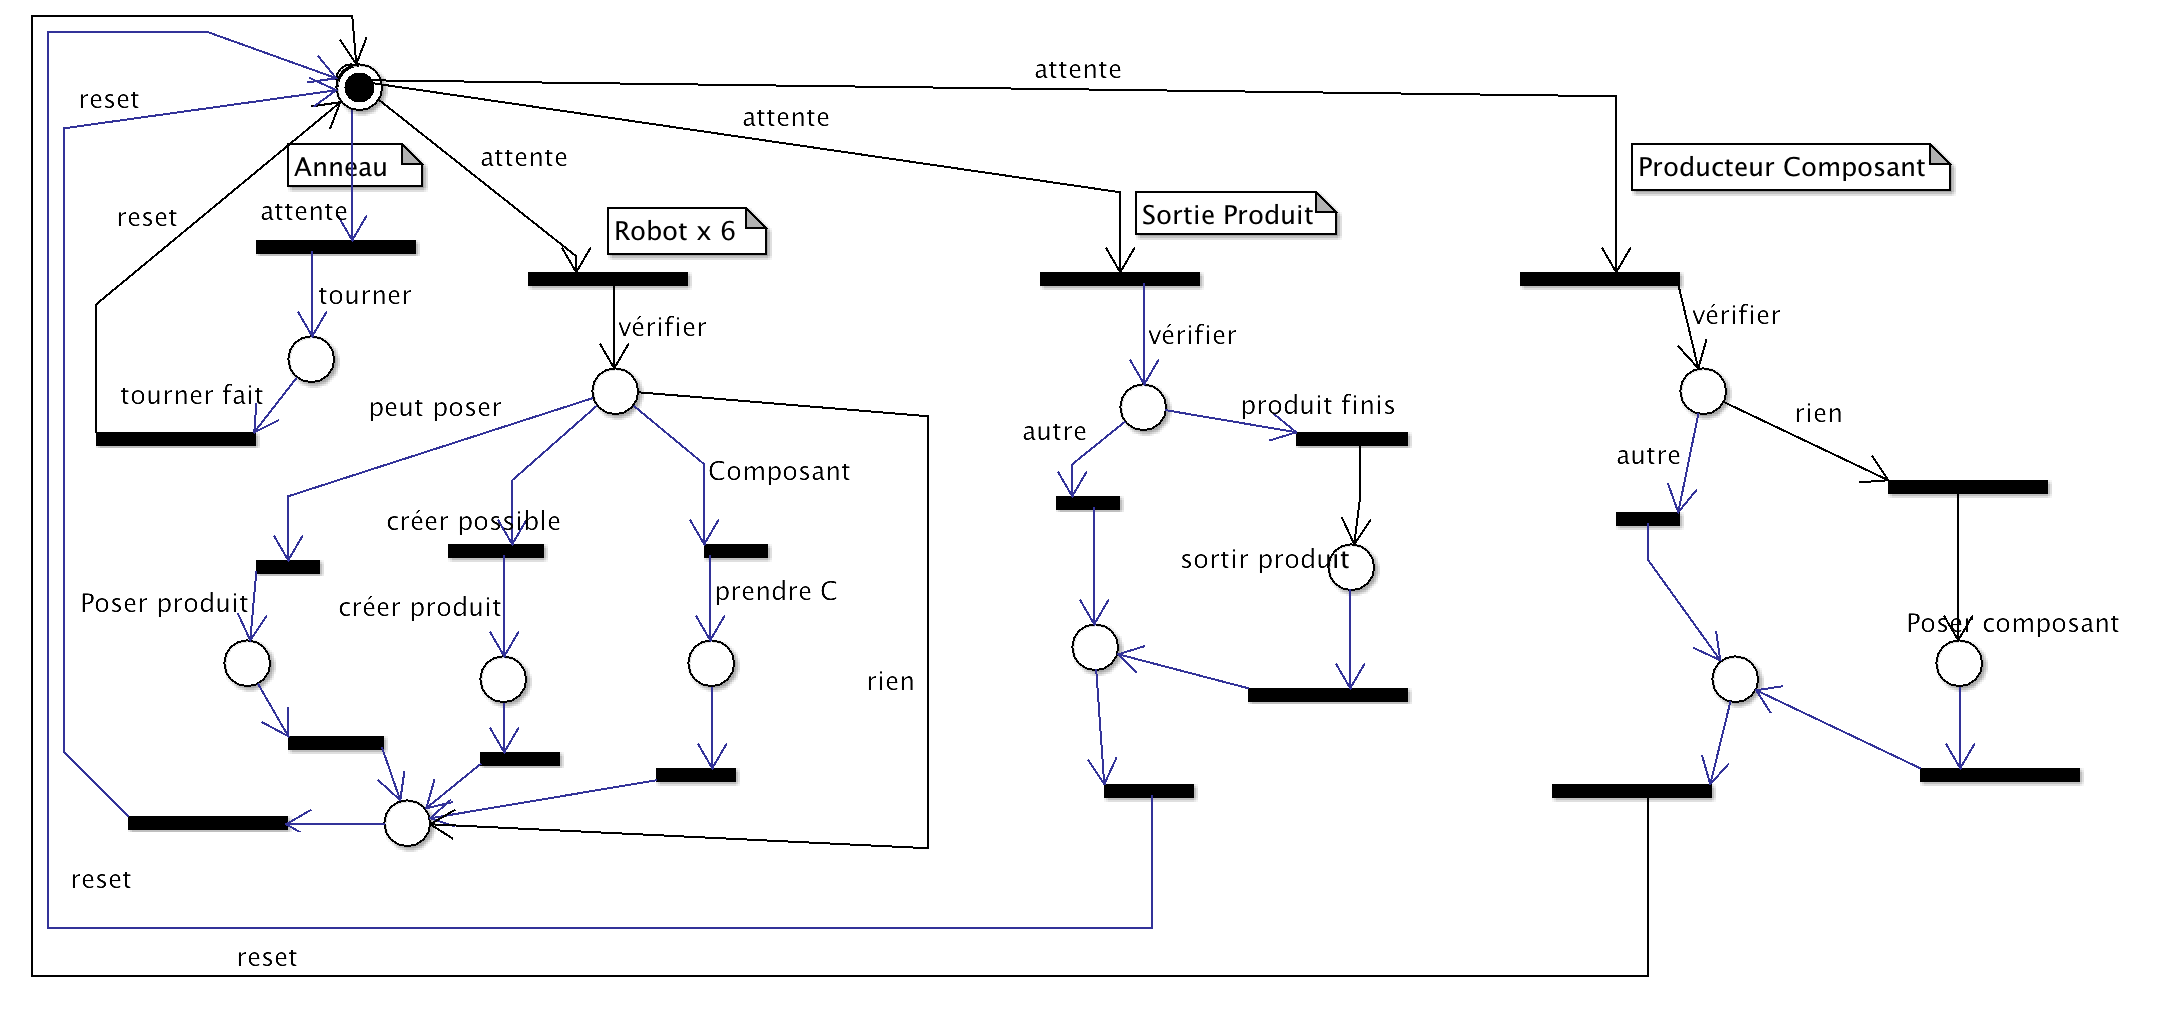
\includegraphics[angle=90,width=320pt]{rdp.png}
\end{figure}

\chapter{Conclusion}
Ce projet a permis de mettre en place plusieurs notions vues en cours, TD et TP, et même d'aller plus loin avec les Factory. De plus il possible de mettre une quantité de composants bien supérieur à ce qui était demandé au minimum (103 composants à la base), il est possible d'en avoir une infinité grâce à notre architecture du programme.\\
Ainsi on a pu utiliser nos connaissances et les approfondir.\\


Pour terminer, nous pensons avoir atteint les objectifs qui étaient fixés : 
\begin{itemize}
\item Code modulable
\item Threads ou processus
\item Synchronisation\\
\end{itemize}


Nous en retirons une bonne expérience et trouvons le sujet intéressant et extrêment bien dosé dans sa complexité, sa longueur et son application du cours.

\appendix
\chapter{Documentation}
%Voici des documents qui m'ont été utiles et fut aussi dans le passé (pour d'autres projets) pour m'amener à réaliser ce projet.
\section{Factory Pattern}

\href{http://fr.wikipedia.org/wiki/Fabrique_(patron_de_conception)}{Wikipedia Fabrique: Patron de conception} (http://fr.wikipedia.org/wiki/Fabrique\_(patron\_de\_conception))


\href{http://design-patterns.fr/fabrique}{Une explication plus poussée} (http://design-patterns.fr/fabrique)
\section{Mes réalisations (github)}\label{realisation}
Voici une bonne partie de mes réalisations en programmation.
\\
\href{https://github.com/Blackdread/}{Mes réalisations sur GitHub} (https://github.com/Blackdread/)
\\

%\chapter{Exemples de code}


\end{document}